% Created November 2014 by Carl D. Sorensen
% Modified August 2019 by Brian D. Jensen

\documentclass[letterpaper, 11pt, twoside, article]{memoir}


%%% REVISION INFORMATION
%%% Set the date and revision number below to the correct values
\newcommand{\revdate}{15 Nov 2019}
\newcommand{\revnum}{2.0}

%%% The material below should only be modified if you know what you're doing with it!
\setstocksize{11in}{8.5in}
\setlrmarginsandblock{1.5in}{1in}{*}


\setulmarginsandblock{1in}{1in}{*}

\checkandfixthelayout[classic]

\usepackage[T1]{fontenc}
	

%\usepackage{fontspec}
\usepackage{graphicx}
\usepackage{booktabs}
\usepackage{enumitem}
\usepackage{xcolor, colortbl}
\usepackage{array}
\usepackage{calc}
\usepackage[font=small,singlelinecheck=false]{caption}
\usepackage{pdfpages}
\usepackage{mathptmx}
\usepackage[hidelinks]{hyperref}

% Add new lists -- Primary Artifacts and Supporting Artifacts
%
%% Primary Artifacts
\newcommand{\primaryartifactname}{Primary Artifacts}
\newlistof{listofprimaryartifacts}{pa}{\primaryartifactname}
\newcounter{primaryartifact}[chapter]
\newlistentry{primaryartifact}{pa}{0}
\renewcommand{\theprimaryartifact}{\arabic{primaryartifact}}
\newcommand{\primaryartifact}[1] {
  \refstepcounter{primaryartifact}
  \addcontentsline{toc}{primaryartifact}{\hspace{1.5em}#1}
  \addcontentsline{pa}{primaryartifact}{\hspace{1.5em}#1}
  }
\cftpagenumbersoff{primaryartifact}  

%% Supporting Artifacts
\newcommand{\supportingartifactname}{Supporting Artifacts}
\newlistof{listofsupportingartifacts}{sa}{\supportingartifactname}
\newcounter{supportingartifact}[chapter]
\newlistentry{supportingartifact}{sa}{0}
\renewcommand{\thesupportingartifact}{\arabic{supportingartifact}}
\newcommand{\supportingartifact}[1] {
  \refstepcounter{supportingartifact}
   \addcontentsline{toc}{supportingartifact}{\hspace{1.5em}#1}
   \addcontentsline{sa}{supportingartifact}{\hspace{1.5em}#1}
  }
\cftpagenumbersoff{supportingartifact}  


% Trick for fixed-width table columns
\newcolumntype{L}[1]{>{\raggedright\let\newline\\\arraybackslash\hspace{0pt}}p{#1}}
\newcolumntype{C}[1]{>{\centering\let\newline\\\arraybackslash\hspace{0pt}}p{#1}}
\newcolumntype{R}[1]{>{\raggedleft\let\newline\\\arraybackslash\hspace{0pt}}p{#1}}

% Fractional Width columns
\newcolumntype{z}[1]{>{\hsize=#1\hsize\raggedright\arraybackslash}X}
\newcolumntype{a}[1]{>{\hsize=#1\hsize\raggedleft\arraybackslash}X}
\newcolumntype{q}[1]{>{\hsize=#1\hsize\centering\arraybackslash}X}

\title{Template for the Opportunity Development Stage Approval Package}
\author{Brian D. Jensen \\ David G. Long \\ Brian A. Mazzeo \\ Carl D. Sorensen }
\date{\revdate \\ Revision \revnum}

%%% This ends the material you should only modify if you know what you're doing.



%%%%% adjust spacing -- Choose one line to uncomment

%\abnormalparskip{0.5\baselineskip}  %adjusts spacing between paragraphs under user control
%\nonzeroparskip  % Default value for non-zero spacing between paragraphs
\traditionalparskip  % No extra spacing between paragraphs -- recommended by Wilson, the author of the memoir class


% Degree symbol
\usepackage{gensymb}
\usepackage{float}

\begin{document}
\raggedbottom
\raggedright

\frontmatter




\begin{centering}
\thispagestyle{empty}

{\Huge Team Objective and Development Overview}

\Large
\vspace{0.5in}
\revdate\\
Revision \revnum
\vspace{0.5in}

% Replace the line below with your project title
Tracker for In-Flight Air Vehicle\\
\vspace{0.5in}

Project Sponsor: \\
 IMSAR

\vspace{0.5in}

% logo

\includegraphics[width=.2\textwidth]{Images/logo_navy.png}

\vspace{0.4 in}

Capstone Team 15: RPS


\normalsize

\vspace{1.6 in}

%\begin{centering}

\Large

Ira A. Fulton College of Engineering \\
Brigham Young University

\end{centering}


\clearpage

\chapter*{Revision History}

\begin{tabularx}{\textwidth}{|q{.3}|q{.5}|z{2.2}|}
\hline
Revision & Date & Description\\
\hline
1.0 & 11 Sept 2019 & Initial Release \\
\hline
1.1 & 18 Sept 2019 & First Draft for Review \\
\hline
1.2 & 30 Sept 2019 & Second Draft, Updated based on feedback from Design Review \\
\hline
1.3 & 1 Oct 2019 & Updated based on feedback from Brian Jensen\\
\hline
1.4 & 2 Oct 2019 & Fixed Typos, and made major updates to requirements matrix, rewrote key success measures based on feedback\\
\hline
1.5 & 3 OCT 2019 & Rewrote Key Success Measures based on a phone meeting with Mark\\
\hline
2.0 & 15 NOV 2019 & Draft for Concept Development; changed date of Concept Development in Project Approval Matrix; updated Project Background to reflect feedback from OD stage; updated Key Success Measures\\
\hline

\end{tabularx}

\cleardoublepage

\begin {centering}
{\LARGE Approval Signatures}

\vspace{.5in}

The undersigned certify that they have read the stage approval package and approve of the requirements and key success measures contained in it.


\end{centering}
\vspace{.5 in}			
\begin{tabularx}{\textwidth}{C{.25 in} L{2.5 in} C{.5 in} R{1.5 in}}
\cline{2-2} \cline {4-4}

& Autumn Twitchell & & Date \vspace{.25 in}\\
\cline{2-2} \cline {4-4}
& Daniel Sharp & & Date \vspace {.25 in}\\
\cline{2-2} \cline {4-4}
& Garret Gang & & Date \vspace{.25 in}\\
\cline{2-2} \cline {4-4}
& Jesse Krage & & Date \vspace{.25 in}\\
\cline{2-2} \cline {4-4}
& Joe Hansen & & Date \vspace{.25 in}\\
\cline{2-2} \cline {4-4}
& Nicholas Merriman & & Date \vspace{.25 in}\\
\cline{2-2} \cline {4-4}
&  Larkin Hastriter - Team Coach & & Date \vspace{.25 in}\\
\cline{2-2} \cline {4-4}
& Mark Catanzaro - IMSAR & & Date \vspace{.25 in}\\
\cline{2-2} \cline {4-4}
& Brian Jensen - Project Instructor & & Date \vspace{0 in}\\

\end{tabularx}

\vspace{1 in}

% why?
%\cleardoublepage
\clearpage

\tableofcontents*


\mainmatter

%\chapter{Contact Information}

\begingroup
\makeatletter
\setlength{\@fptop}{0pt}
\setlength{\@fpbot}{0pt plus 1fil}
\makeatother
\begin{table}[p]
{


\chapter{Contact Information}
    \renewcommand{\arraystretch}{1.5}
    \centering
    \begin{tabularx}{1.0\textwidth}{l l l l}
        \hline
        Name & Title & Cell Phone & Email \\
        \hline
        \hline
         Autumn Twitchell & EE Student & 801-388-5666 & atwitch23@gmail.com\\
         Daniel Sharp & EE Student & 801-888-6053 & danielsharp.a@gmail.com \\
        Garret Gang & CE Student & 520-333-0168 & garretgang@gmail.com\\
        Jesse Krage & EE Student & 619-878-4245 & jessekrage5@gmail.com \\
        Joe Hansen & ME Student & 208-850-7781 & 1joehansen@gmail.com \\
        Nicholas Merriman & ME Student & 385-240-3759 & nicholas.merriman95@gmail.com\\
        Larkin Hastriter & Team Coach & 937-979-3481 & larkinhastriter@yahoo.com \\
        \newline
    \end{tabularx}
    {
    \begin{center}
    \textbf{IMSAR Contact Information}
    \end{center}
    }
    \begin{tabularx}{1.0\textwidth}{l l l l}
        \hline
        Name & Title & Office Phone & Email \\
        \hline
        \hline
        Daniel Gunyan & VP of Engineering & 801-798-8440 & dgunyan@imsar.com\\
        Mark Catanzaro & Verification Engineer & 801-798-8440 & markc@imsar.com 
    \end{tabularx}
    }
\end{table}
    \clearpage
\endgroup



%\includepdf[pages = {1}, pagecommand =\chapter{Contact Information}, offset = 0 -1.5cm]{contact_info.pdf}


\chapter{Project Background}

% Project Background

IMSAR is a local company based out of Springville, UT, that specializes in making compact radar systems more affordable and accessible for use in small air vehicles. Since their conception in 2004, they have fulfilled multiple contracts with the Department of Defense and have developed radar systems with applications ranging from fighting fires to detecting enemy troop movements.
~\\~\\
One of the radar positioning systems (RPS) currently produced and sold by IMSAR is a computer-controlled tilt and pan positioner that maintains a communication link with radar units installed on air vehicles. The operational situation for these units is to be in a stationary position 2 to 20 miles away from the target in-flight vehicle. The current design employs a tilt and pan positioner that has become obsolete. The goal of this project is to replace the tilt and pan positioner, install an onboard computer, and to improve upon the current design. The current design requires that the data processing be done remotely on an external machine and has a barely passable user interface. Our final design will eliminate the need for external data processing. Challenges include integrating a new onboard control computer and proper handshaking between subsystems. The new RPS will be tested against IMSAR's drones flying in the vicinity. We will validate system functionality by tracking the drone with a camera mounted to the RPS. IMSAR will provide the positioning gimbal, and as such designing a positioner is not within the scope of our project.\\

{
\begin{figure}[H]
\begin{center}

\captionsetup{justification=centering,margin=2cm}
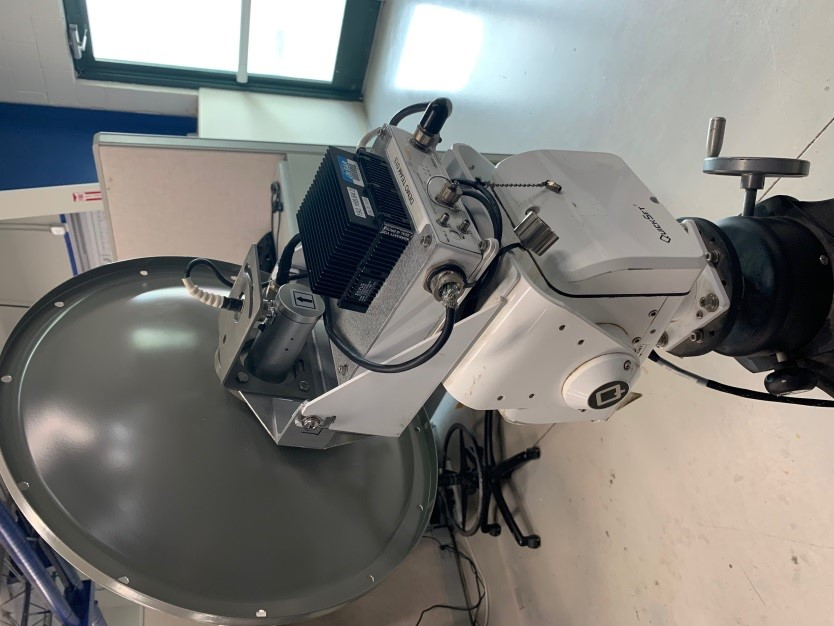
\includegraphics[angle=-90]{Images/IMSAR_PositioningSystem.jpg}
\caption{Current IMSAR Positioning System}
\end{center}
\end{figure}
}


\clearpage

\chapter{Project Objective Statement}

% Project Objective Statement

The team will design, prototype, and test a Radar Positioning System (RPS) that can track in-flight vehicles while maintaining visual contact by March 30th 2020 for under \$1,500 USD and 1,500 man hours. 


\chapter{Project Approval Matrix}

 %% Project Approval Matrix

    \begin{center}
    \label{tab:Approval_Matrix}
    \begin{tabular}{ >{\raggedright}p{2.4cm} p{2.3cm} >{\raggedright}p{6.5cm} r}

    \hline
    \textbf{Development Stage}& \textbf{Expected Completion Date} & \textbf{Artifacts Required for Approval} & \textbf{Budget} \\

    \hline
    \hline
    Opportunity Development & 19 Sept 2019 & Team Objective and Development Overview, System Requirement Matrix with sections A-D completed, Requirement Validation & \$5\\
    &&&\\
    Concept\\ Development & 22 Nov 2019 & Written and Visual Definition of Concept, Concept Selection Report, Requirements Matrix with Target Values, Revised TODO, Concept Testing Reports & \$590\\
    &&&\\
     Architecture\\ Review & 10 Jan 2020 & System Architecture Document, System Requirements Matrix, Architecture Justification Document & \$5\\
    &&&\\
    Subsystem\\ Engineering & 14 Feb 2020 & System Design Package, System Requirements Matrix, Measured and Predicted Performance Summary & \$400\\
    &&&\\
    System\\ Refinement & 27 Mar 2020 & Written and Visual Description of Design, Performance Summary, System Requirements Matrix & \$200\\
    &&&\\
    Final\\ Reporting & 2 Apr 2020 & Fully Transferable Design, Functioning Prototype, Final Capstone Report & \$300\\
    \hline
    \end{tabular}
    \end{center}

   
   \break
%\chapter{Key Success Measures}


\chapter{Key Success Measures}
{
    \centering
   \resizebox{\textwidth}{!}
    {
    \begin{tabular}{>{\raggedright}p{3cm} >{\raggedright}p{2cm} >{\raggedright}p{2.3cm} >{\raggedright}p{2.3cm} >{\raggedright}p{2.2cm} >{\raggedright}p{1.2cm}  p{1.5cm} p{1.7cm}}
    
    \hline
   \textbf{Measure} & \textbf{Stretch Goal} & \textbf{Excellent Performance} & \textbf{Good Performance} & \textbf{Fair Performance} & \textbf{Lower Limit} & \textbf{Ideal} & \textbf{Upper Limit} \\
    \hline
    \hline
    
    
    
    Time to Train User &
    N/A &
    5 minutes &
    10 minutes &
    20 minutes &
    N/A &
    5 minutes &
    30 minutes \\
    
    \hline
    
    Percent Increase in Target Aquistion Time from Minimum Aquistion Time &
    10\% &
    20\% &
    30\% &
    40\% &
    N/A &
    0\% &
    50\% \\
    
    \hline
    
    Initial Setup Time &
     2 minutes &
     5 minutes &
     7 minutes &
     9 minutes &
     N/A &
     2 minutes &
     10 minutes\\
    
    \hline    
    
    \\
    
 \end{tabular}
 }
 }
 The key success measures shown above were chosen to help determine the desirability of the radar posititioning system (RPS). They will distinguish our design from a basic, functioning design. By achieving excellence in our key success measures we expect to exceed the customer's expectations. The team feels that these goals define our highest quality of work. Our key success measures account for the major flaws in IMSAR's current system. The user interface and setup time have caused the most issues for IMSAR and as such they drive our key succes measures. Reasoning for our defined measurements is given below.
 ~\\~\\
  The interface is currently barely usable and by running a survey and testing the interface with market representatives we intend to deliver an interface that does not require extensive training. It also takes a long time (10 minutes) to setup the RPS on site, due to the complexity of entering the data to control the RPS. We aim to reduce this by making it easier to enter the information and by improving the usage of non-volatile memory. The usage cases of IMSAR's radar units specify that every second matters when reacquiring the communication link. Mark was supportive of these key success measures and he participated in a team call in which we decided these key success measures (see NOTE-003).
  ~\\~\\


     
\chapter{Summary of Requirement Validation}

% Summary of Requirement Vailidation

The requirements matrix (see REQ-001 artifact) is a result of direct feedback from IMSAR's VP of Engineering, Daniel Gunyan, and Project Engineer Lead, Mark Catanzaro. In our first meeting with Daniel, we learned more about the scope of the project, and generated a rough outline of market requirements and some performance measures.  After that meeting, we drafted the first iteration of our requirements matrix that we presented in person to Mark the following week.  As part of this meeting with Mark, we were able to see the current system in use, and address a variety of questions (see NOTE-001). After our discussion, Mark made minor changes to our performance measures, and gave us approval for the matrix via email (see REQ-002).
~\\~\\
Since gaining Mark's initial approval, we have made changes to both the market requirements and the performance measures for improved clarity and measurability. We have stayed in contact with Mark via phone calls and emails during the revision process. In our most recent discussion with Mark, we went over our key success measures and he approved of them (see NOTE-003).\\

  
\chapter{Change Management Procedure}

% Change Management Procedure

When it is determined that the TODO requires a revision, an engineering change order must be filled out (See ECO-000). The proposer will be the ECO owner. The proposer should include a description and justification of the proposed changes.
~\\~\\
A completed copy of the ECO and TODO will be presented to the members of the team. When team feedback is implemented a completed copy will be sent to contacts at IMSAR for approval, after  IMSAR's approval we will send the revision to Dr. Jensen for approval. For the proposed changes to be approved and implemented three signatures are required: The capstone team leader, a pod instructor, and a representative from IMSAR. Once the ECO is approved the proposed changes will be made to the TODO, and the revision history table filled out. If the ECO is rejected, no changes will be made. 

   
\addtocontents{toc} {
\cftpagenumbersoff{chapter}  % turn off page numbers in TOC
\cftpagenumbersoff{section}
}

%\cleardoublepage
\clearpage
\pagestyle{empty}



\clearpage

\end{document}
